\section{Problem Formulation and Learning Model}
\label{sec:formulation}

\begin{figure}[h]
	\begin{center}
		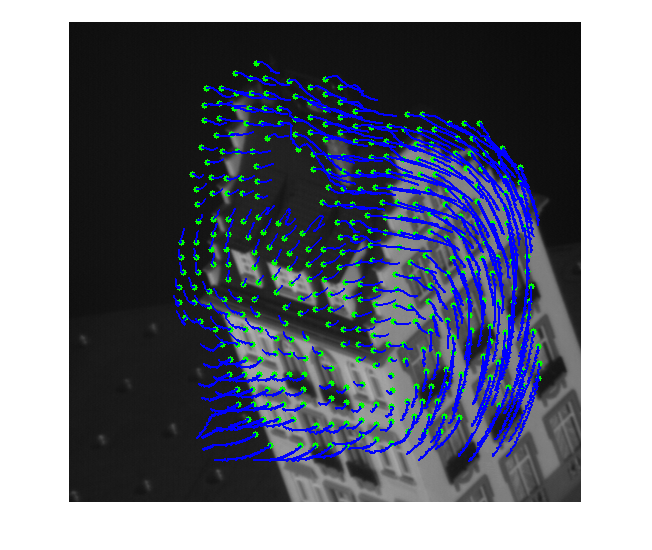
\includegraphics[width=2.5in]{figs/hotel-traces.png}
	\end{center}
	\caption{Example of traces from SIFT and KLT}
	\label{fig:traces}
\end{figure}


We use SIFT features and the KLT matching algorithm to track a set of features
through time.  The particular parameters of the tracking and matching phases
depend on application.  Our learning algorithm operates directly on the output
of KLT.  The features are represented as a set of $P$ feature traces across $F$
frames where each trace comprises two $F\times 1$ vectors,
\begin{align*}
x = (x_1, \ldots, x_F)\tr && y = (y_1, \ldots, y_F)\tr
\end{align*}
which together trace out the screen-space location of tracked points.  
In Figure \ref{fig:traces}, we see an example of overlaying the traces from KLT
on the first image in a sequence.  As was mentioned previously, our goal is
detect traces that are outliers.  We define outliers to be traces whose {\it
shape} is largely different than the shape of the other traces in the image.
For example, in Figure \ref{fig:colored-traces}(a), we note that some traces,
such as the red ones on the carpet, look quite different from the traces on the
chair.

Therefore, in order to compare trace shape we compare the velocity of the
tracked features at given points in time.
%We are not interested in the location of tracked features as much as their velocity at
%given points in time, which corresponds to the shape of the traces.  
This differential is recovered by finding the movement of each point relative
to the previous frame:
\begin{align*}
\dot x = (x_2-x_1, \ldots, x_F-x_{F-1})\tr && \dot y = (y_2-y_1, \ldots, y_F-y_{F-1})\tr
\end{align*}
We assume in our model that motion of each trace is independent in its two
axes, and that the motions at any two points in time are independent.  This
assumption is highly reasonable for traces resulting from the unsteadiness of a
handheld camera, and is necessarily true if fast twitch motions occur within
the sampling frequency of the camera.  Thus, for each tracked feature point, we
can form a $2(F-1)\times 1$ vector, called the {\it trace differential vector}:
\begin{align*}
\dot w = \left( \begin{array}{c}\dot x \\ \dot y\end{array} \right)
\end{align*}
Once we've calculated the trace differential vectors, $\{\dot w_1, \dot w_2,
\ldots , \dot w_P\}$, for each of $P$ tracked points, we need a model to
differentiate ``normal'' and outlier traces.
Noting that it's possible for the set of valid traces to be split into several
distinct clusters (for example, the different faces of an object or different
objects in a scene), we decided to use a mixture model.  Because of the
aforementioned independence assumptions, a naive Bayes Gaussian mixture model (GMM)
is sufficient.  
Once we have trained our GMM, we can ``score'' each trace differential, giving it a
probability of being part of any mixture in the GMM.  We use the
log-probability from the trace differential as an indicator of the likelihood
that any given trace is an outlier.  This relatively simple model and the
resulting probabilities turn out to be quite useful for a number of tasks.

%train some sort of
%statistical model on the entire set.  With the trained model, we calculate the
%log-probability of each trace differential vector and interpret that as an
%outlier-score for the feature trace, with lower scores corresponding to more
%likely outliers.  The question then remains what sort of model to use.  
%Noting that it's possible for the set of valid traces to be split into several
%distinct clusters (for example, those correspondnig to different faces of an
%object), we decided to use a mixture model.  Because of the aforementioned
%independence assumptions, a naive bayes gaussian mixture model is sufficient.  

Having implemented this exact model on one of the homework assignments, we
decided to avoid numerical precision risks and use MATLAB's implementation,
which employs the expectation maximization algorithm.  In all of our
experiments, four mixture elements seems to produce reasonable results,
although this number might benefit from tweaking.  For stability reasons, a
small amount of regularization on the variance parameter is also required.
Since the resulting score of the model is very sensitive to the random
initialization of expectation maximization, we perform the entire train/score
sequence many times, and average the results in log-space.  In our experiments,
100 iterations averaged was sufficiently fast and produced little variance in score
between runs.
